%% -*- coding: utf-8 -*-
\documentclass[12pt,a4paper]{scrartcl} 
\usepackage[utf8]{inputenc}
\usepackage[english,russian]{babel}
\usepackage{indentfirst}
\usepackage{misccorr}
\usepackage{graphicx}
\usepackage{amsmath,amsfonts,amssymb,amsthm,mathtools} % It`s AMS
\begin{document}
	\begin{titlepage}
		\begin{center}
			\large
			МИНИСТЕРСТВО НАУКИ И ВЫСШЕГО ОБРАЗОВАНИЯ РОССИЙСКОЙ ФЕДЕРАЦИИ
			
			Федеральное государственное бюджетное образовательное учреждение высшего образования
			
			\textbf{АДЫГЕЙСКИЙ ГОСУДАРСТВЕННЫЙ УНИВЕРСИТЕТ}
			\vspace{0.25cm}
			
			Инженерно-физический факультет
			
			Кафедра автоматизированных систем обработки информации и управления
			\vfill

			\vfill
			
			\textsc{Отчет по практике}\\[5mm]
			
			{\LARGE Вариант 7. \textit{Найти определитель матрицы.}}
			\bigskip
			
			2 курс, группа 2ИВТ
		\end{center}
		\vfill
		
		\newlength{\ML}
		\settowidth{\ML}{«\underline{\hspace{0.7cm}}» \underline{\hspace{2cm}}}
		\hfill\begin{minipage}{0.5\textwidth}
			Выполнил:\\
			\underline{\hspace{\ML}} А.\,В.~Масалов\\
			«\underline{\hspace{0.7cm}}» \underline{\hspace{2cm}} 2021 г.
		\end{minipage}%
		\bigskip
		
		\hfill\begin{minipage}{0.5\textwidth}
			Руководитель:\\
			\underline{\hspace{\ML}} С.\,В.~Теплоухов\\
			«\underline{\hspace{0.7cm}}» \underline{\hspace{2cm}} 2021 г.
		\end{minipage}%
		\vfill
		
		\begin{center}
			Майкоп, 2021 г.
		\end{center}
	\end{titlepage}

% Что должно быть во введении
% Содержание
\section{Введение}
\label{sec:intro}


Целью данной работы является написание программы для нахождение определителя матрицы.

Определителем квадратной матрицы $A=\left(\begin{array}{cc}a_{11}&a_{12}\\a_{21}&a_{22}\end{array}\right)$ второго порядка называется число |$A|=a_{11}a_{22}-a_{12}a_{21}$.\\

Определителем $A=\left(\begin{array}{ccc}a_{11}&\cdots&a_{1n}\\\vdots&\ddots&\vdots\\a_{n1}&\cdots&a_{nn}\end{array}\right)$ квадратной матрицы порядка $n,n\geq3$, называется число $|A|=\Sigma^{n}_{k=1}(-1)^{k+1}a_{1k}M_{k}$, где $M_{k}$ - определитель матрицы порядка $n-1$, полученной из матрицы $A$ вычеркиванием первой строки и столбца с номером $k$.

\section{Ход работы}
\label{sec:exp}

\subsection{Код приложения}
\label{sec:exp:code}
\begin{verbatim}
#include<iostream>
using namespace std;
void PrintMatr(int** mas, int m) {
    int i, j;
    for (i = 0; i < m; i++) {
        for (j = 0; j < m; j++)
            cout << mas[i][j] << " ";
        cout << endl;
    }
}
void GetMatr(int** mas, int** p, int i, int j, int m) {
    int ki, kj, di, dj;
    di = 0;
    for (ki = 0; ki < m - 1; ki++) { 
        if (ki == i) di = 1;
        dj = 0;
        for (kj = 0; kj < m - 1; kj++) { 
            if (kj == j) dj = 1;
            p[ki][kj] = mas[ki + di][kj + dj];
        }
    }
}
int Determinant(int** mas, int m) {
    int i, j, d, k, n;
    int** p;
    p = new int* [m];
    for (i = 0; i < m; i++)
        p[i] = new int[m];
    j = 0; d = 0;
    k = 1; 
    n = m - 1;
    if (m < 1) cout << "Определитель вычислить невозможно!";
    if (m == 1) {
        d = mas[0][0];
        return(d);
    }
    if (m == 2) {
        d = mas[0][0] * mas[1][1] - (mas[1][0] * mas[0][1]);
        return(d);
    }
    if (m > 2) {
        for (i = 0; i < m; i++) {
            GetMatr(mas, p, i, 0, m);
            cout << mas[i][j] << endl;
            PrintMatr(p, n);
            d = d + k * mas[i][0] * Determinant(p, n);
            k = -k;
        }
    }
    return(d);
}
int main() {
    int m, i, j, d;
    int** mas;
    system("chcp 1251");
    system("cls");
    cout << "Введите размерность квадратной матрицы: ";
    cin >> m;
    mas = new int* [m];
    for (i = 0; i < m; i++) {
        mas[i] = new int[m];
        for (j = 0; j < m; j++) {
            cout << "mas[" << i << "][" << j << "]= ";
            cin >> mas[i][j];
        }
    }
    PrintMatr(mas, m);
    d = Determinant(mas, m);
    cout << "Определитель матрицы равен " << d;
    cin.get(); cin.get();
    return 0;
}
\end{verbatim}

\section{Пример вставки изображения}
\label{sec:picexample}

\begin{figure}[h]
	\centering
	
	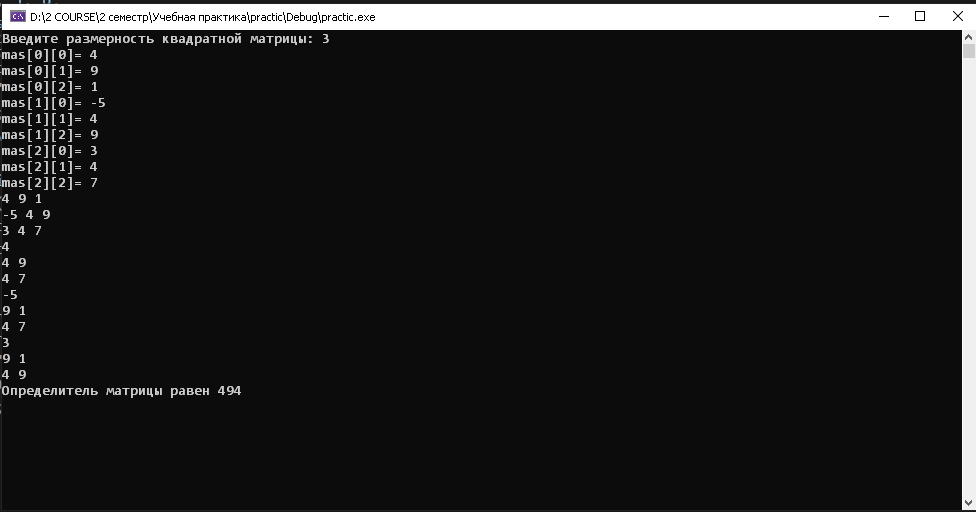
\includegraphics[width=1\textwidth]{prog.png}
\end{figure}

\begin{thebibliography}{9}
\bibitem{Knuth-2003}Кнут Д.Э. Всё про \TeX. \newblock --- Москва: Изд. Вильямс, 2003 г. 550~с.
\bibitem{Lvovsky-2003}Львовский С.М. Набор и верстка в системе \LaTeX{}. \newblock --- 3-е издание, исправленное и дополненное, 2003 г.
\bibitem{Vorontsov-2005}Воронцов К.В. \LaTeX{} в примерах 2005 г.
\end{thebibliography}

\end{document}
